\section{Prozess}

Die Erarbeitung unserer Ideen erfolgte im Rahmen eines Design Thinking Prozesses in zwei Schritten:

\begin{enumerate}
\item Bestimmung einer Persona
\item Ideengenerierung
\end{enumerate}

Die Leitung des Design Thinking Prozesses hat Philipp übernommen. Wir haben zunächst eine Persona aufgestellt, die aus zehn Kategorien (zum Beispiel demographische Daten, Interessen und Lifestyle) bestand. Dazu hat sich jedes Teammitglied individuell Gedanken gemacht und diese auf Post-Its festgehalten (\ref{fig:design_thinking:01}). Anschließend haben wir die Ideen gesammelt und in der Gruppe diskutiert (\ref{fig:design_thinking:02}). Zur Vollendung der Persona wurden dann die unserer Meinung nach wichtigsten Merkmale herausgefiltert.
 
\begin{figure}[h]
\centering
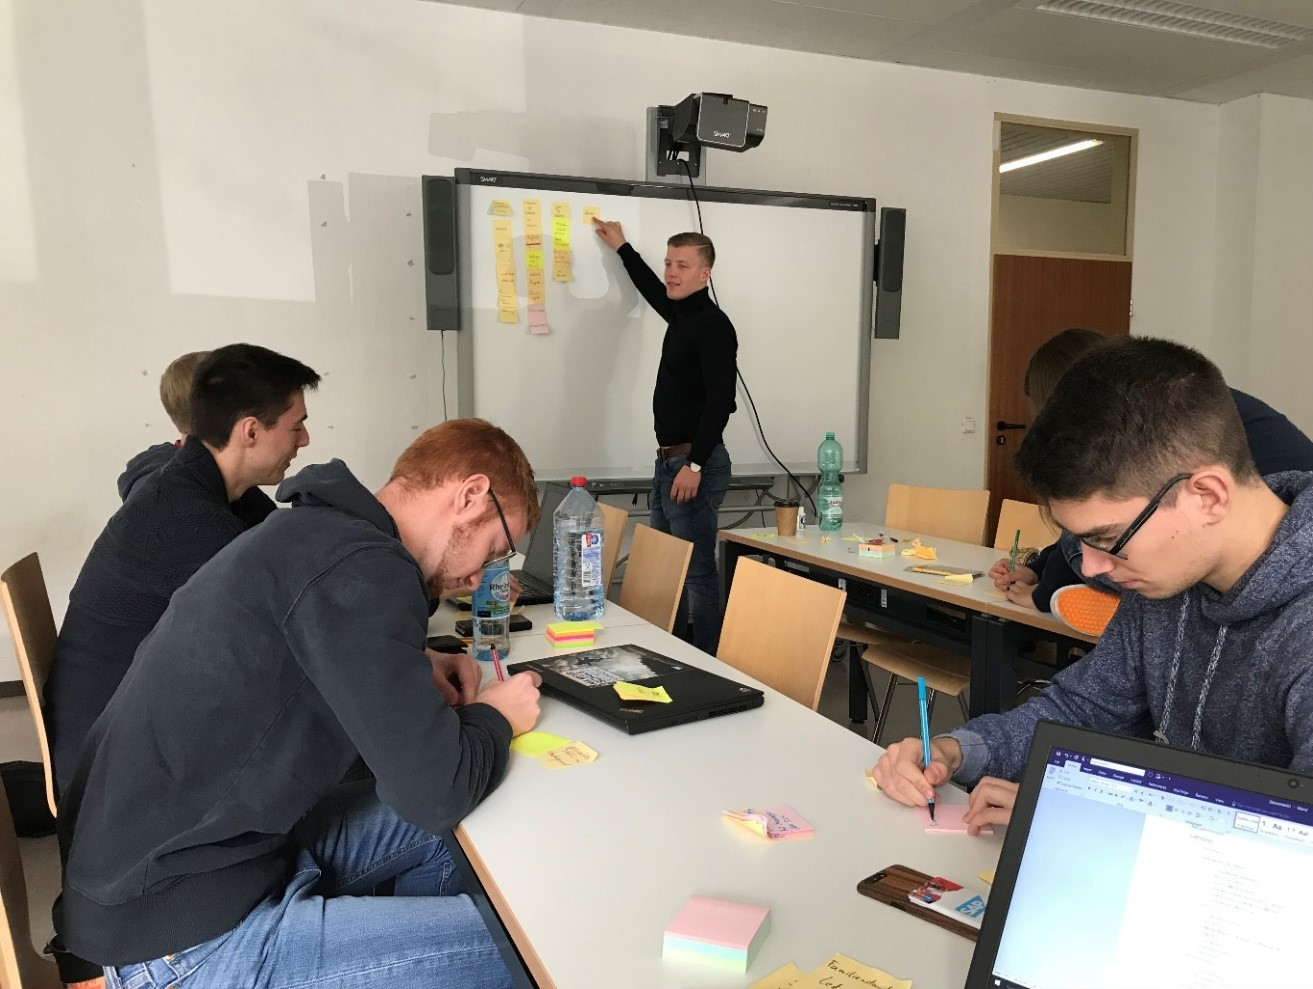
\includegraphics[width=0.8\textwidth]{images/design_thinking/01}
\caption[Erarbeitung der Eigenschaften zur Persona]{Erarbeitung der Eigenschaften zur Persona}
\label{fig:design_thinking:01}
\end{figure}
 
\begin{figure}[h]
\centering
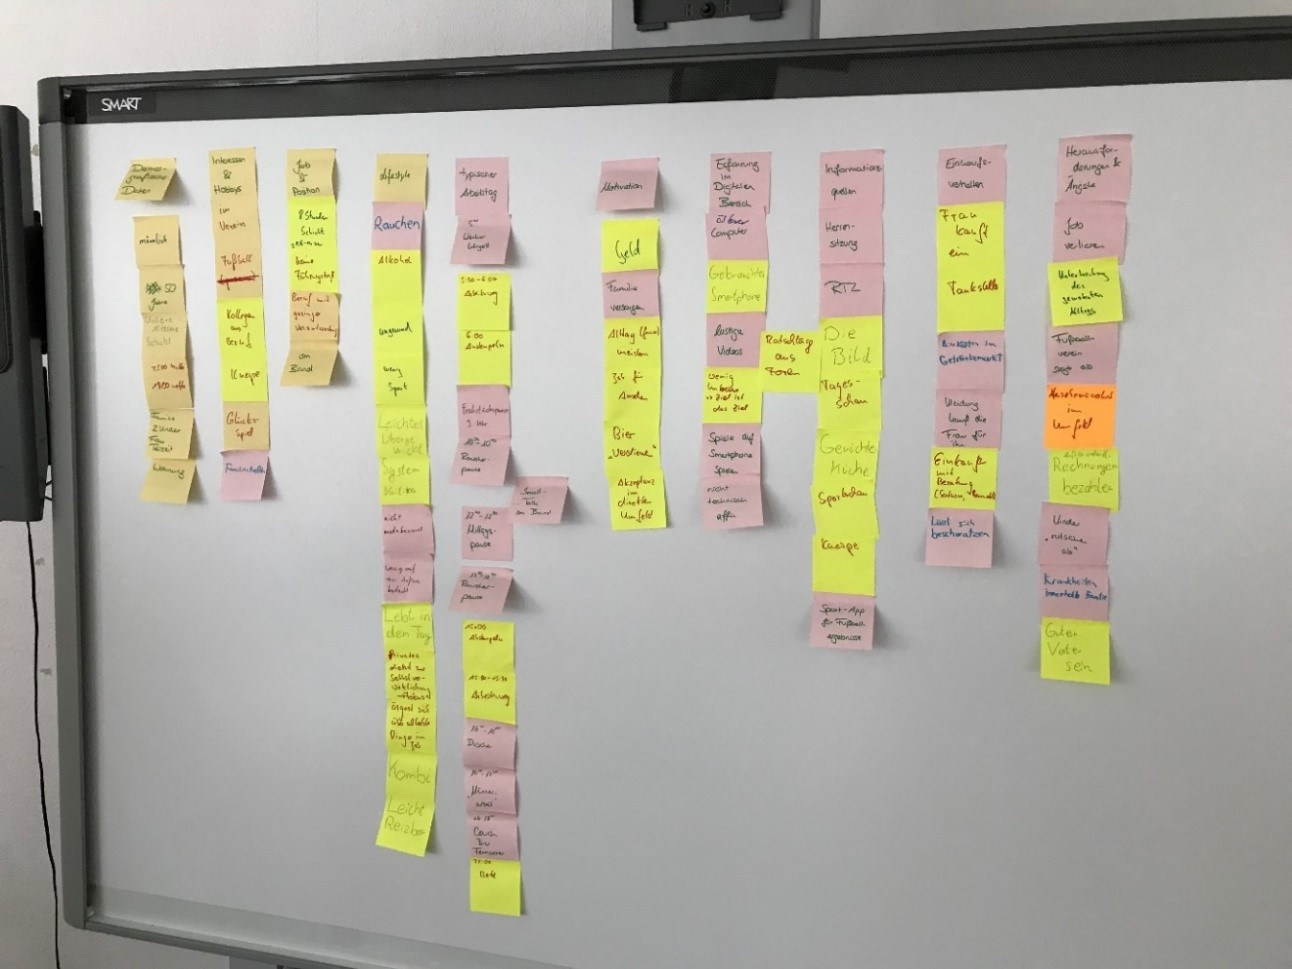
\includegraphics[width=0.8\textwidth]{images/design_thinking/02}
\caption[Gesammelte Eigenschaften der Persona]{Gesammelte Eigenschaften der Persona}
\label{fig:design_thinking:02}
\end{figure}
 
Zum Zweck der Ideengenerierung wurde im Anschluss ein Brainstorming durchgeführt, wobei jeder seinen Gedanken freien Lauf lassen konnte. Jeder Einfall und jede Idee wurden, egal wie abstrus sie ist, auf Post-Ist an die Tafel geklebt (\ref{fig:design_thinking:03}). Daraufhin haben wir gemeinsam Gruppen aus den bislang ungeordneten Ideen gebildet und darüber diskutiert (\ref{fig:design_thinking:04}). Auf Basis der Gruppen konnten wir dann konkrete Konzepte für die Umfrage im Unternehmen entwickeln. Die Konzepte wurden anschließend in Teams aus zwei bis drei Leuten ausgearbeitet.
 
\begin{figure}[h]
\centering
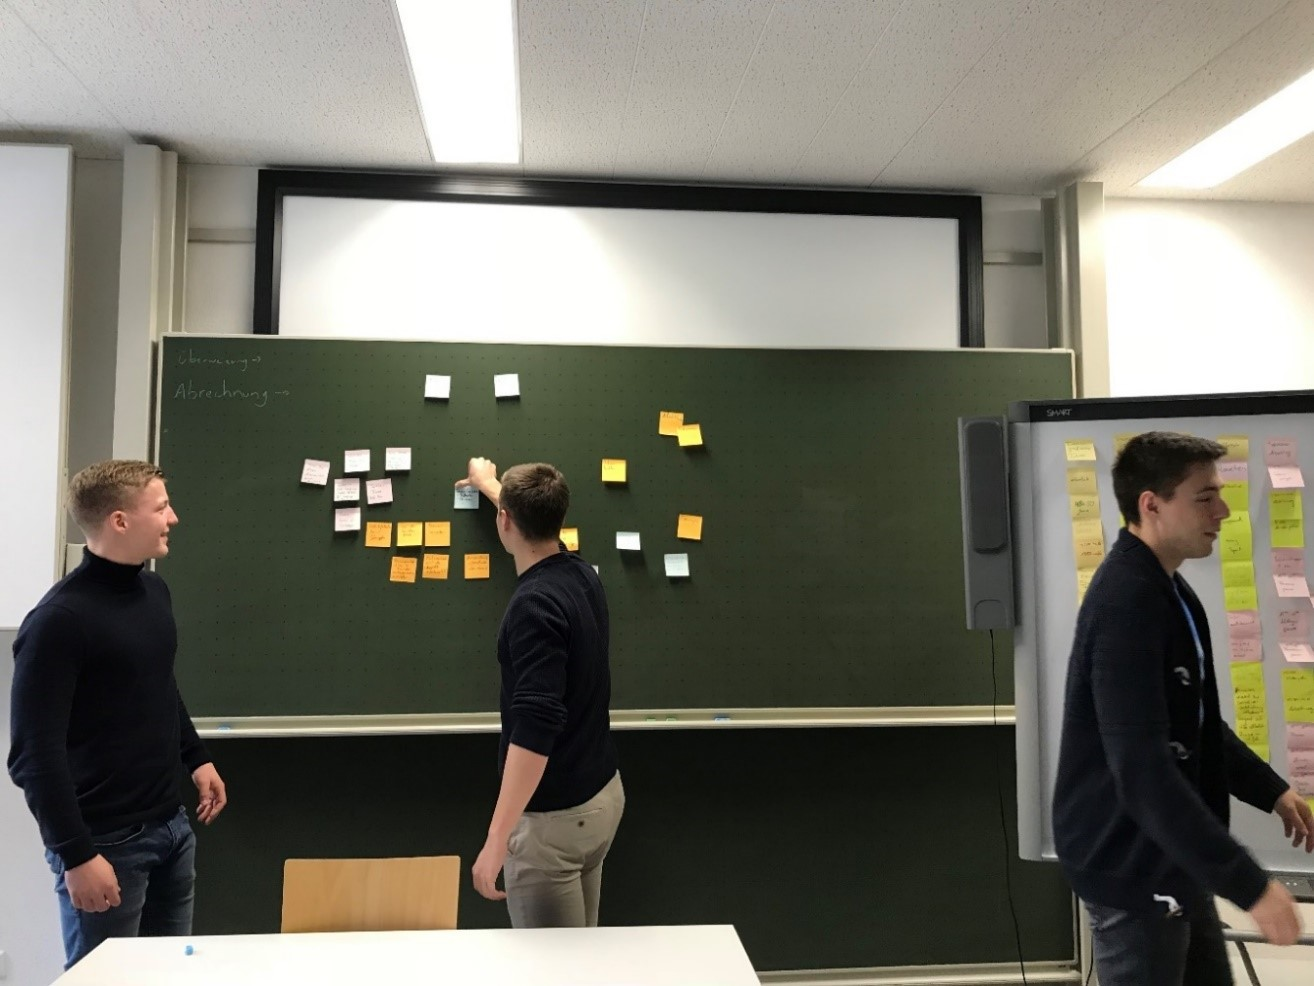
\includegraphics[width=0.8\textwidth]{images/design_thinking/03}
\caption[Brainstorming]{Brainstorming}
\label{fig:design_thinking:03}
\end{figure} 

\begin{figure}[h]
\centering
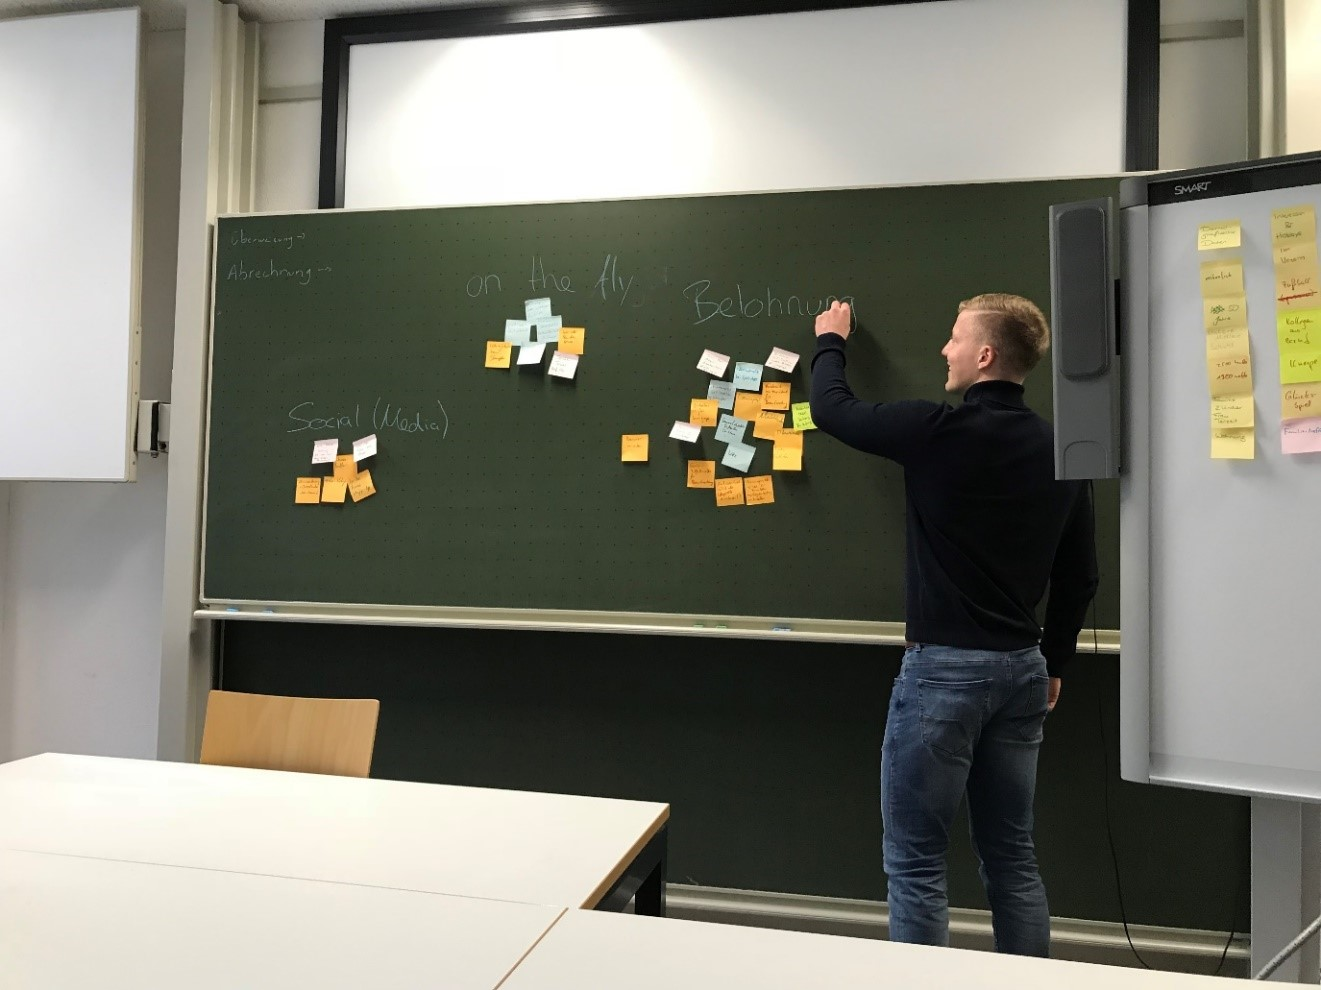
\includegraphics[width=0.8\textwidth]{images/design_thinking/04}
\caption[Gruppenbildung]{Gruppenbildung}
\label{fig:design_thinking:04}
\end{figure} 
 